\documentclass[border=20pt]{standalone}
\usepackage{tikz}
\usepackage{amsmath}
\usetikzlibrary{calc,arrows.meta}
\begin{document}
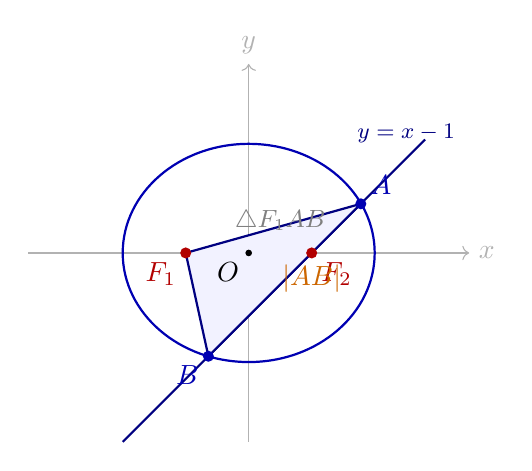
\begin{tikzpicture}[scale=0.8]
  % Axes
  \draw[->, gray!60, thin] (-3.5,0) -- (3.5,0) node[right] {$x$};
  \draw[->, gray!60, thin] (0,-3.0) -- (0,3.0) node[above] {$y$};

  % Ellipse: x^2/4 + y^2/3 = 1, a=2, b=√3≈1.732, c=1
  \draw[thick, blue!70!black] (0,0) ellipse (2 and 1.732);

  % Foci
  \coordinate (F1) at (-1, 0);
  \coordinate (F2) at (1, 0);
  \coordinate (O)  at (0,0);

  % Line through F2 with slope 1: y = x - 1
  % Intersection with 3x^2 + 4y^2 = 12:
  % 3x^2 + 4(x-1)^2 = 12 → 3x^2 + 4x^2 - 8x + 4 = 12 → 7x^2 - 8x - 8 = 0
  % x = (8±√(64+224))/14 = (8±√288)/14 = (8±12√2)/14 = (4±6√2)/7
  % x1 ≈ 1.78, x2 ≈ -0.64
  \coordinate (A) at (1.78, 0.78);
  \coordinate (B) at (-0.64, -1.64);

  % The line through F2
  \draw[thick, blue!50!black] (-2.0, -3.0) -- (2.8, 1.8);
  \node[blue!50!black, font=\footnotesize] at (2.5, 1.9) {$y=x-1$};

  % Triangle F1-A-B
  \draw[thick, blue!50!black, fill=blue!5] (F1) -- (A) -- (B) -- cycle;

  % Points
  \fill[red!70!black]  (F1) circle (2.5pt) node[below left]  {$F_1$};
  \fill[red!70!black]  (F2) circle (2.5pt) node[below right] {$F_2$};
  \fill[blue!70!black] (A)  circle (2.5pt) node[above right] {$A$};
  \fill[blue!70!black] (B)  circle (2.5pt) node[below left]  {$B$};
  \fill[black]         (O)  circle (1.5pt) node[below left]  {$O$};

  % Labels
  \node[orange!80!black] at (1.0, -0.4) {$|AB|$};
  \node[gray, font=\small] at (0.5, 0.5) {$\triangle F_1AB$};
\end{tikzpicture}
\end{document}
